\documentclass{standalone}
\usepackage{tikz}
\usetikzlibrary{math}

\begin{document}
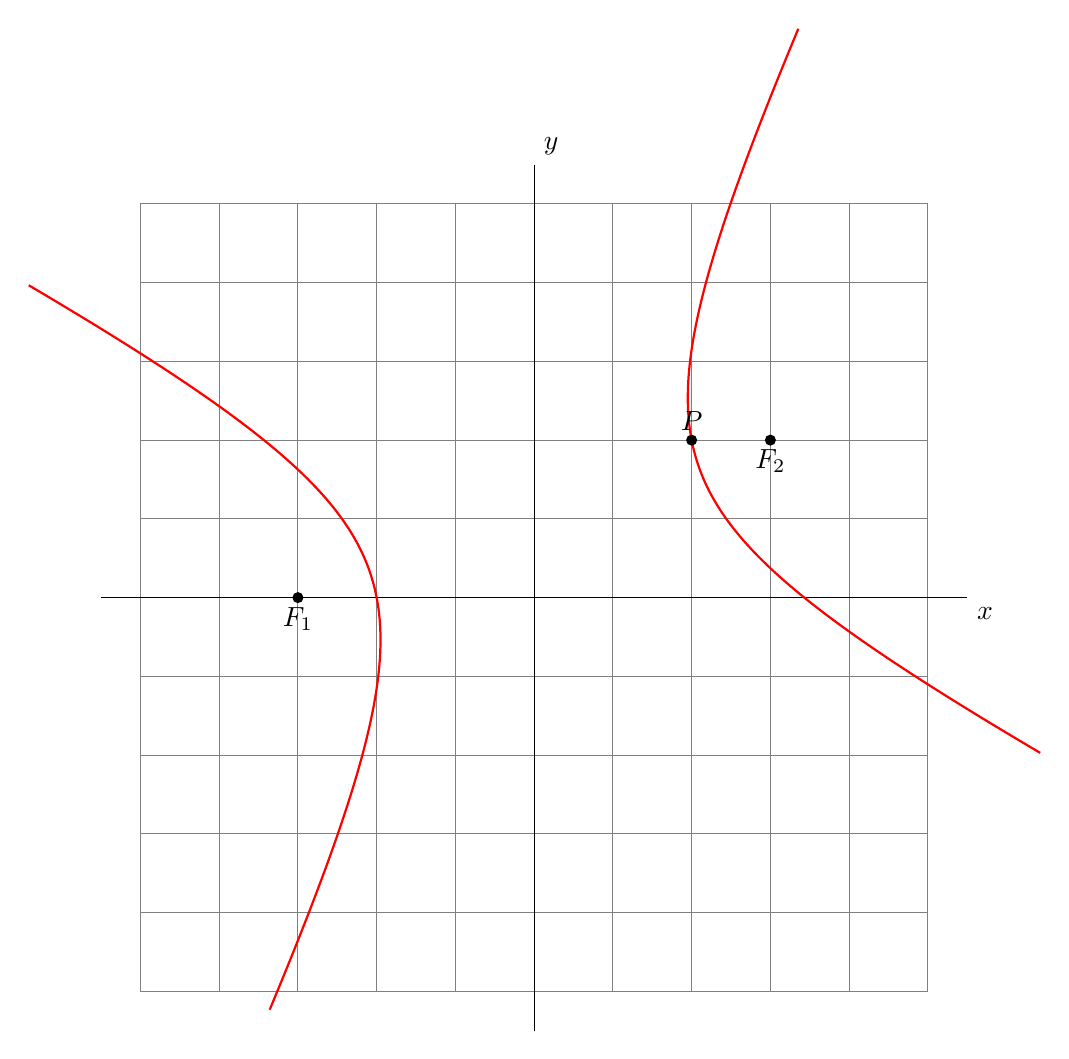
\begin{tikzpicture}
    % 定义输入:焦点 Fa, Fb 和双曲线上一点 P
    \def\xFa{-3}    \def\yFa{0}   % 焦点 Fa 坐标
    \def\xFb{3}    \def\yFb{2}   % 焦点 Fb 坐标
    \def\xP{2}     \def\yP{2}    % 点 P 在双曲线上

    % 计算双曲线参数
    \tikzmath{
        % 中心 (h, k)
        \h = (\xFa + \xFb)/2; \k = (\yFa + \yFb)/2;
        % 焦距 c
        \c = sqrt((\xFb - \h)^2 + (\yFb - \k)^2);
        % 计算实半轴 a
        \dPFa = sqrt((\xP - \xFa)^2 + (\yP - \yFa)^2);  % 点 P 到 Fa 的距离
        \dPFb = sqrt((\xP - \xFb)^2 + (\yP - \yFb)^2);  % 点 P 到 Fb 的距离
        \a = abs(\dPFa - \dPFb) / 2;
        % 虚半轴 b
        \b = sqrt(\c^2 - \a^2);
        % 旋转角度 θ(焦点连线与 x 轴的夹角)
        \angle = atan2(\yFb - \yFa, \xFb - \xFa);    
    }

    \draw[gray] (-5,-5) grid (5,5);
    \draw (-5.5, 0) -- (5.5, 0) node[below right] {$x$};
    \draw (0, -5.5) -- (0, 5.5) node[above right] {$y$};

    % 使用 insert path 绘制双曲线
    \draw[red, thick, insert path={
        [rotate around={\angle:(\h,\k)}]  % 绕中心旋转 θ
        % 右分支
        plot[domain=-1.5:1.5, smooth, samples=100] 
            ({\h + \a*cosh(\x)}, {\k + \b*sinh(\x)})
        % 左分支
        plot[domain=-1.5:1.5, smooth, samples=100] 
            ({\h - \a*cosh(\x)}, {\k + \b*sinh(\x)})
    }];

    % 标出焦点和点 P
    \fill (\xFa,\yFa) circle (2pt) node[below] {$F_1$};
    \fill (\xFb,\yFb) circle (2pt) node[below] {$F_2$};
    \fill (\xP,\yP) circle (2pt) node[above] {$P$};
\end{tikzpicture}
\end{document}